\documentclass[twoside,11pt]{article}

%================================ PREAMBLE ==================================

%--------- Packages -----------
\usepackage{fullpage}
\usepackage{amssymb}
\usepackage{amsmath}
\usepackage{amsthm}
\usepackage{latexsym}
\usepackage{graphicx}
\usepackage{wrapfig}
\usepackage{color}
\usepackage{url}
%\usepackage{algorithm,algorithmic}
\usepackage{nn-macros}
\usepackage{subcaption}
%---------- Spacing ----------
\setlength{\parindent}{0pt}
\setlength{\parskip}{8pt}
\geometry{margin=0.7in}
%---------Definitions----------
\newcommand{\half}{{\textstyle{\frac{1}{2}}}}
\renewcommand{\>}{{\rightarrow}}
\renewcommand{\hat}{\widehat}
\renewcommand{\tilde}{\widetilde}
\newcommand{\grad}{{\nabla}}
%
\newcommand{\argmax}{\textup{\textrm{argmax}}}
\newcommand{\argmin}{\textup{\textrm{argmin}}}
\newcommand{\argsort}{\textup{\textrm{argsort}}}
\newcommand{\sign}{\textup{\textrm{sign}}}
\newcommand{\poly}{\textup{\textrm{poly}}}
\newcommand{\er}{\textup{\textrm{er}}}
\newcommand{\zo}{\textup{\textrm{0-1}}}
\newcommand{\sq}{\textup{\textrm{sq}}}
%
\newcommand{\1}{{\mathbf 1}}
\newcommand{\0}{{\mathbf 0}}
\newcommand{\I}{{\mathbf I}}
\newcommand{\R}{{\mathbb R}}
\newcommand{\Z}{{\mathbb Z}}
\newcommand{\N}{{\mathbb N}}
\renewcommand{\P}{{\mathbf P}}
\newcommand{\E}{{\mathbf E}}
\newcommand{\Var}{{\mathbf{Var}}}
%
\renewcommand{\a}{{\mathbf a}}
\renewcommand{\b}{{\mathbf b}}
\renewcommand{\c}{{\mathbf c}}
\renewcommand{\d}{{\mathbf d}}
\newcommand{\f}{{\mathbf f}}
\renewcommand{\k}{{\mathbf k}}
\newcommand{\p}{{\mathbf p}}
\newcommand{\q}{{\mathbf q}}
\renewcommand{\u}{{\mathbf u}}
\newcommand{\w}{{\mathbf w}}
\newcommand{\x}{{\mathbf x}}
\newcommand{\y}{{\mathbf y}}
%
\newcommand{\A}{{\mathbf A}}
\newcommand{\bC}{{\mathbf C}}
\newcommand{\C}{{\mathcal C}}
\newcommand{\cD}{{\mathcal D}}
\newcommand{\F}{{\mathcal F}}
\renewcommand{\H}{{\mathcal H}}
\newcommand{\K}{{\mathbf K}}
\renewcommand{\L}{{\mathcal L}}
\newcommand{\bL}{{\mathbf L}}
\newcommand{\cN}{{\mathcal N}}
\newcommand{\W}{{\mathbf W}}
\newcommand{\X}{{\mathcal X}}
\newcommand{\bX}{{\mathbf X}}
\newcommand{\Y}{{\mathcal Y}}
%
\newcommand{\bloss}{{\boldsymbol \ell}}
\newcommand{\blambda}{{\boldsymbol \lambda}}
\newcommand{\bmu}{{\boldsymbol \mu}}
\newcommand{\bnu}{{\boldsymbol \nu}}
\newcommand{\bSigma}{{\boldsymbol \Sigma}}
\newcommand{\seta}{{\boldsymbol \eta}}
\newcommand{\bpsi}{{\boldsymbol \psi}}
\newcommand{\bphi}{{\boldsymbol \phi}}
\newcommand{\bPhi}{{\boldsymbol \Phi}}
\newcommand{\balpha}{{\boldsymbol \alpha}}
\newcommand{\bxi}{{\boldsymbol \xi}}

%=============================== END PREAMBLE ===============================

\begin{document}

%================================ COVER PAGE ================================

%*********** Use this for project proposal (comment out in project report) ************
\emph{\footnotesize{CIS 520 Spring 2019, Project Report}}

%*********** Use this for project report (comment out in project proposal) ************
%\emph{\footnotesize{CIS 520 Spring 2018, Project Report}}

\vspace{12pt}

%Fill in your project title
\textbf{\Large{Fatal or Non-fatal: Comparative Study of 
		Classification Algorithms \\for Cardiac Arrhythmias 
		Discrimination}}

\vspace{1cm}

\textbf{Team Members:}

\begin{tabular}{lll}%{@{}l l l}
	Al\"{e}na Rodionova & 
	(PennKey: nellro &
	Email: 
	\href{mailto:nellro@seas.upenn.edu}{nellro@seas.upenn.edu}) \\
	%
	Haochen Han & 
	(PennKey: hanhc& 
	Email: \href{mailto:hanhc@seas.upenn.edu}{hanhc@seas.upenn.edu})\\
	%
	Haotian Zhu &
	(PennKey: htzhu& 
	Email: \href{mailto:htzhu@seas.upenn.edu}{htzhu@seas.upenn.edu})\\
	%
	Po-Yuan Wang & 
	(PennKey: poyuanw & 
	Email:
	\href{mailto:poyuanw@seas.upenn.edu}{poyuanw@seas.upenn.edu})
\end{tabular}

%---

\vspace{2cm}

%*********** Comment out the following for the proposal; uncomment and fill in all details for the project report ***********

\textbf{Assigned Project Mentor:}

%Fill in assigned TA name
Brandon Lin

\vspace{1cm}

\textbf{Team Member Contributions:}

%Fill in team member contributions
\begin{center}
	\begin{tabular}{|c|c|}
		\hline
		\textbf{Team member} & \textbf{Contributions} \\ \hline
		Al\"{e}na Rodionova&   Problem formulation, data 
		pre-processing (feature extraction), DNN methodology\\ 
		\hline
		Haochen Han&    Decision tree methodoloy, result analysis \\ 
		\hline
		Haotian Zhu&    SVM methodoloy, FFT feature extraction, FFT 
		approach  \\ \hline
		Po-Yuan Wang&  kNN methodology, modified kNN approach  \\ 
		\hline
	\end{tabular}
\end{center}

\vspace{12pt}

\textbf{Code Submission:}

\url{https://github.com/nellro/CIS520_project}


\newpage
%
\section{Introduction}
\label{sec:intro}
In this project we compared classification methods for 
electrogram (EGM) arrhythmia discrimination. The set of methods we 
analysed include Deep Neural Network (DNN), Support Vector Machine 
(SVM), $k$-Nearest Neighbours (\knn) and Decision Tree.

\section{Data}
The following two datasets were used: 
\begin{itemize}
%	\item \href{https://physionet.org/physiobank/database/mitdb/}{The 
%	MIT-BIH Arrhythmia Database}~\cite{moody2001impact}. 
%	It contains $48$ half-hour two-channel ECG recordings, obtained 
%	from $47$ subjects. The 
%	recordings are digitized at $360$ samples per second. 
%	There are approximately $110,000$ ECG
%	beats. 
%	in this database with $15$ different types of arrhythmia 
%including normal.
%	The subjects were 25 men aged 32 to 89 years, and 22 women aged 
%	23 to 89 years.
	\item Cardiac model EGM database~\cite{jiang2016silico}. 
	% EGM - cardiac device incoming cardiac voltage signal
	It consists
	of $1920$ EGM signals, equally split into $960$ VTs and
	$960$ SVTs. The EGMs were generated by the heart
	model that has been validated for realism by 
	cardiologists~\cite{jiang2016silico}.
	\item Ann Arbor Electrogram Libraries~\cite{egm_data}. It 
	consists of 89 EGM recordings: 62 VT signals and 27 SVT signals. 
	Signals are of different length, varying from 10 seconds to 2 
	minutes recordings. 
\end{itemize}

Data pre-processing, following the methodology 
from~\cite{hajeb2018automated}, includes the following steps:
\begin{enumerate}
	\item Resample each signal with a sampling frequency of $300$Hz.
	\item Filter the signal with a fourth-order bandpass Butterworth 
	filter with low cut-off frequency of $0.4$Hz and high cut-off 
	frequency of $40$Hz to avoid baseline drift and reduce 
	high-frequency noise. 
	\item Segment the signal into $10$s data lengths.
	\item Extract 6 features from each signal (6 for each V signal 
	and 6 for each A signal, 12 in total): four features are derived 
	from image-based phase plot analysis 
	(see~\cite{hajeb2018automated}), one derived in the 
	frequency domain (number of frequencies which have higher 
	amplitude than the mean value), and the last feature is Shannon 
	Entropy~\cite{shannon1948mathematical} (The SE value is higher 
	for VT than for SVT).
\end{enumerate}

\section{Related work}
\label{sec:related}
Describe related previous work, including citations to references

\cite{qres_ama}, \cite{DBLP:journals/pieee/AbbasAMMR18}
\section{Data set}
\label{sec:data}

\begin{figure}[t]
	\centering
	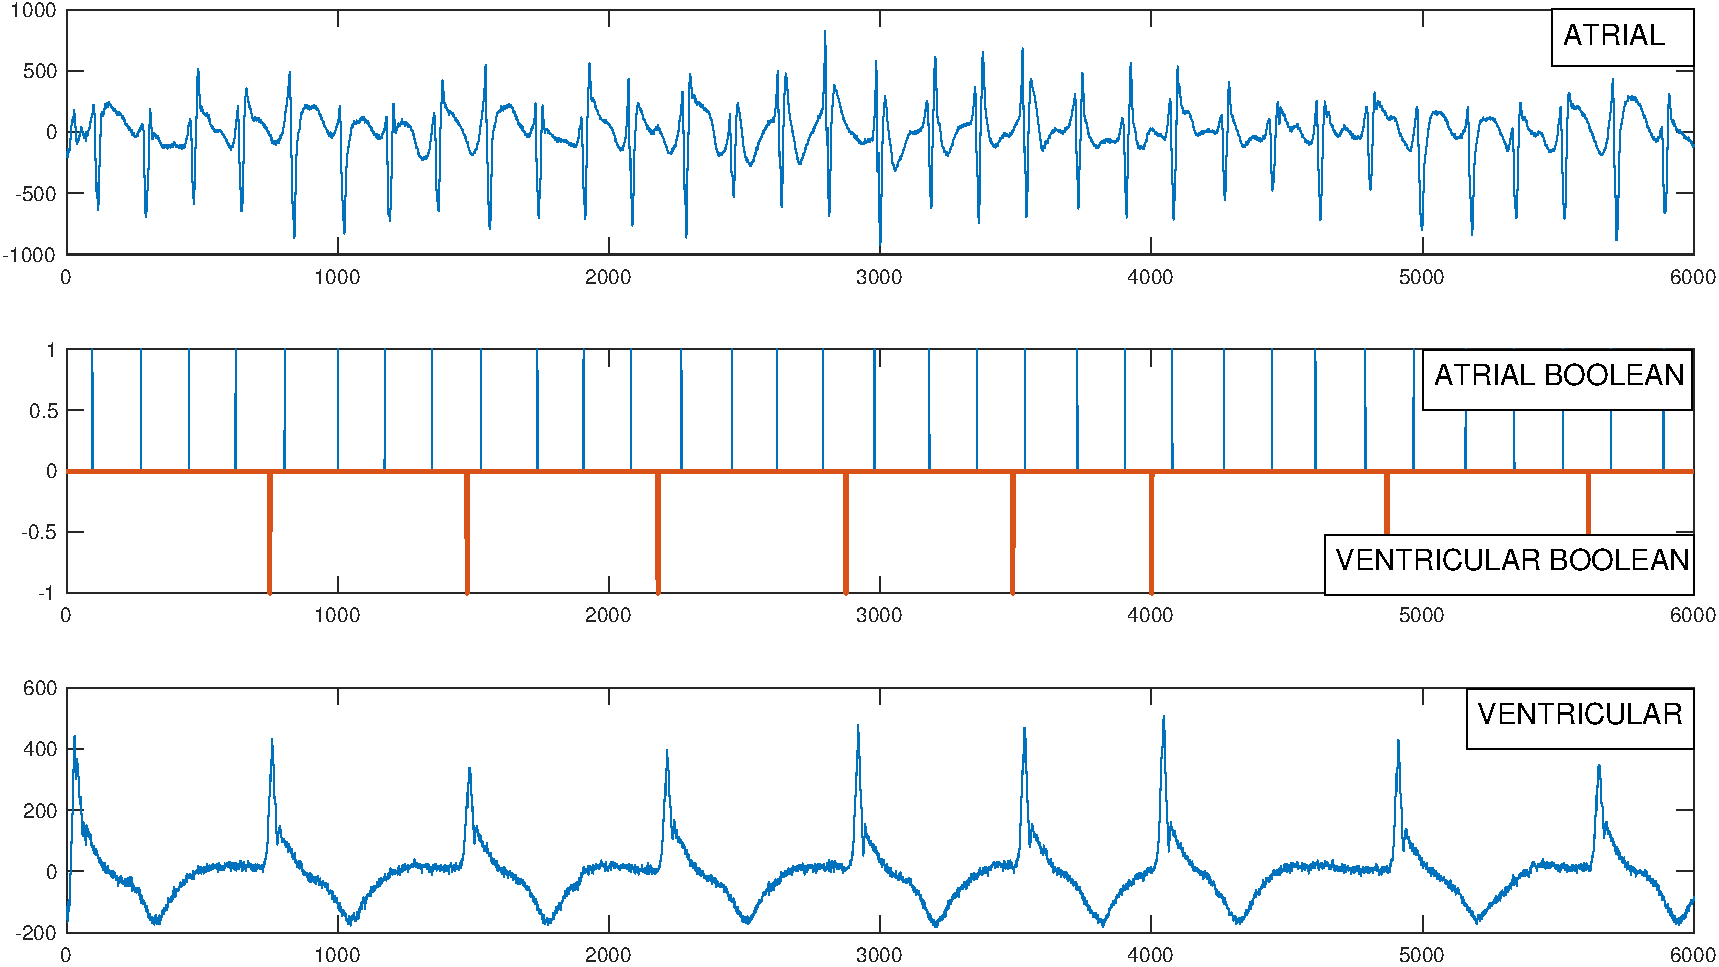
\includegraphics[scale=0.3]{figures/atachs.pdf}
	\caption{EGM recording during SVT. Bottom panel represents 
	V-signal, top 
	panel shows A-signal, middle panel presents corresponding 
	boolean beat channels.}
	\label{fig:egm}
\end{figure}

For our problem we used the  
%	\item \href{https://physionet.org/physiobank/database/mitdb/}{The 
%	MIT-BIH Arrhythmia Database}~\cite{moody2001impact}. 
%	It contains $48$ half-hour two-channel ECG recordings, obtained 
%	from $47$ subjects. The 
%	recordings are digitized at $360$ samples per second. 
%	There are approximately $110,000$ ECG
%	beats. 
%	in this database with $15$ different types of arrhythmia 
%including normal.
%	The subjects were 25 men aged 32 to 89 years, and 22 women aged 
%	23 to 89 years.
\textbf{Cardiac Model EGM Database}~\cite{jiang2016silico}. 
The EGM (electrogram) signals in the database were generated 
by the heart
model that has been validated for realism by 
cardiologists~\cite{jiang2016silico}.
	% EGM - cardiac device incoming cardiac voltage signal
	The database consists
	of $1920$ EGMs, equally split into $960$ VTs 
	and
	$960$ SVTs. Each recording has two real-valued channels, 
	depending on the 
	heart chamber where they were measured: Ventricular channel 
	(V-signal) and Atrial channel (A-signal). Each recording also has 
	two boolean channels, representing the detected heart beats in V- 
	and A-signals.
	
	An example SVT EGM recording is shown in a Figure~\ref{fig:egm}. 

%	\item Ann Arbor Electrogram Libraries~\cite{egm_data}. It 
%	consists of 89 EGM recordings: 62 VT signals and 27 SVT signals. 
%	Signals are of different length, varying from 10 seconds to 2 
%	minutes recordings. 
%\end{itemize}
\subsection{Data pre-processing and features extraction}
Following the methodology 
from~\cite{hajeb2018automated}, data pre-processing includes the 
following steps:
\begin{enumerate}
	\item Resample each signal with a sampling frequency of $300$Hz.
	\item Filter the signal with a fourth-order bandpass Butterworth 
	filter with low cut-off frequency of $0.4$Hz and high cut-off 
	frequency of $40$Hz to avoid baseline drift and reduce 
	high-frequency noise. 
	\item Segment the signal into $10$s data lengths.
	\item Extract 6 features from each signal (6 for each V-signal 
	and 6 for each A-signal: 12 in total): 
%	\begin{itemize}
%		\item Four features are derived 
%		from image-based phase plot analysis. These features 
%		represent nonlinear and non-stationary dynamics
%		of the signal, see~\cite{hajeb2018automated}.
%		\item One derived in the 
%		frequency domain, and is defined as a number of frequencies 
%		which have higher amplitude than the mean value.
%		\item One feature is Shannon 
%		Entropy~\cite{shannon1948mathematical} (The SE value is 
%		higher for VT than for SVT).
%	\end{itemize}
	four features are derived 
	from image-based phase plot analysis 
	(these features represent nonlinear and non-stationary dynamics
	of the signal, see~\cite{hajeb2018automated}), one derived in the 
	frequency domain (number of frequencies which have higher 
	amplitude than the mean value), and the last feature is Shannon 
	Entropy~\cite{shannon1948mathematical} (The SE value is higher 
	for VT than for SVT).
\end{enumerate}

%The first step of many algorithms that we will implement is feature 
%extraction. For ECG signals, those features can include, but not 
%limited to: signal amplitude, beat duration, signal segments and 
%waves durations, frequency domain features, short beats counter. 
\section{Solution methods}
\label{sec:methods}

The set of methods we analyze implement and compare include: 
\begin{itemize}
	\item Deep Neural Network (DNN) (Al\"ena),
	\item Support Vector Machine (SVM) (Haotian),
	\item $k$-Nearest Neighbours (\knn)(Po-Yuan),
	\item Decision Tree (Haochen).
\end{itemize}

Related work review shows that decision trees can achieve high 
accuracy results in arrhythmia classification based on ECG signals. 
As the database for our project is also in ECG form, decision tree is 
a valid candidate for distinguishing fatal/non-fatal tachycardias. 
Compared with neural networks, decision trees have an advantage that 
it is easy to interpret. 
Unlike neural network, the transparency of decision tree gives us a 
better understanding of the intermediate processes.
 
\knn algorithm is known for its implementation simplicity and fast 
training time. 
It is also robust to noisy data. 
One potential difficulty is that $k-$NN is sensitive to 
irrelevant features. 
The biggest disadvantage of \knn is its expensive computation cost in 
the testing phase. 
Moreover, in case of high-dimensional data, the distance between the 
two data points becomes less meaningful and the accuracy may 
decrease~\cite{beyer1999nearest}. 

%PCA is a commonly used method to compress data and fasten 
%training process, and the data we will use is relatively large in 
%size (about 2MB per instance), so PCA could be useful, especially 
%when the model is not so simple, which requires a lot of calculation.

After accomplishing the main part of our project, we will focus on 
the possible modifications of the algorithms such as cost-sensitive 
decision tree, combining \knn and k-d tree, AdaBoost. 
% that might lead to computational improvements. We will 
\subsection{Deep Neural Network}
\label{sec:dnn}

The proposed DNN model consists of 2 hidden layers with 10 neurons 
each, $12$ 
neurons in the input layer (we use 12 features input data 
representation, see Section~\ref{sec:data}) and one node in the 
output layer, see 
Figure~\ref{fig:dnn_graph}. These hyper-parameters were obtained by 
running the set of experiments and comparing the performance, no 
cross-validation was performed.  

Relu activation functions were used, output layer uses logistic 
sigmoid activation function to produce an estimate of the probability 
of VT label.
At the training phase we minimize the cross-entropy loss 
$l_{\log}:\{0,1\}\times[0,1]\rightarrow\mathbb{R}_{+}$:
\begin{equation}
l_{\log}(y,p)= -y\log p - (1-y)\log(1-p)
\end{equation}
We trained the proposed DNN model for 3000 epochs (one forward and 
backward pass of \textit{all} the training examples) with a batch 
size of 128 (number of training examples in one forward/backward 
pass). 

Implementation results are presented in the Table~\ref{tbl:res}.
\paragraph{Implementation.}
We used Keras 2.2.4, the Python Deep Learning library which runs on 
top of TensorFlow. The Python version is 3.6.
We ran experiments using Ubuntu 18.04 LTS with no GPU support.

\subsection{Decision Tree}
\label{sec:tree}

\subsection{Support Vector Machine}
\label{sec:svm}

We believe that on EGM VT and SVT samples would have very different 
signatures, which makes them separable with linear or other 
relatively “simple” kernels SVM. And the SVM part majorly focus on 
which type of selection of features would give better performance. 
%The raw data is sequences of EGM signal, which are: \\
%1.	Long and large (average about 20000 integers per instance). \\
%2.	For real data set, instances are of different length (because 
%real parents are measured for different length of time), which can 
%vary from 400 to 40000 (integers) per instance. \\
%It’s obvious that raw data’s pre-processing would be necessary. 

In this section we will analyze four methods of features extraction. 
The performance results are presented in the Table~\ref{tbl:svm}. The 
models are all SVM with polynomial kernel, which are determined by 
best their performance. 

First, a na\"ive approach is to pick the time of the heart beat in 
EGM signal. We take first $n$ 
heart beat moments (truncate the heart-beat moment sequence because 
raw data’s difference in length, and in this case 76 integers per 
instance), give extracted data to SVM model. 

Yet just to ignore signal with relatively low intensity causes 
information loss, and additional information could be the key to 
improve model's performance. Section~\ref{sec:data} describes 12 
features with biological meaning that could be used for 
training/testing. Such approach gives better performance than na\"ive 
approach.

In addition, the feature extraction procedures are performed on the 
whole raw data, which is the whole EGM signal within given time 
period, which might take a long time to measure. In real time 
life-or-death situation, even a few seconds could be the difference 
between survival and fatality. We want to find a method which gives 
us acceptable error while time-saving in data pre-processing. So we 
turn to Real Time Fast Fourier Transform. FFT will transform signal 
in time domain to frequency domain, and amplitude represents energy 
of this frequency. A natural idea is to take information of several 
frequencies with highest energy, so that we believe the wave they 
reconstructed is closed enough to original one and information loss 
becomes trivial. So this time the features are the frequency, 
amplitude and phase of $k$ frequencies with highest amplitude (In 
this case, 10 frequencies are chosen). 

And the fourth approach is to use PCA over the spectrum to do the 
frequency-choosing part, rather than pick $k$ frequencies with 
highest amplitude, since data given to model is ``some features of 
many features'' (pick several frequencies among spectrum), which is a 
dimensional reduction task. 

And as shown in chart, if we do not have real-time requirement, 
12-feature is the best; however, FFT with 10 highest frequencies have 
acceptable error when real-time is needed. 

\paragraph{Implementation.}
Parameters for SVM: \\
Use polynomial kernel, pick degree q as an integer in range [2, 4]
\begin{equation*}
G(x_{j},x_{k}) = (1+x_{j}’ x_{k})^{q}
\end{equation*}



\begin{table}[]
	\begin{center}
	\begin{tabular}{|l|l|c|c|c|c|}
		\hline
		\multicolumn{2}{|l|}{}                                        
		                            & 
		\multicolumn{1}{l|}{\textbf{Naive Approach }} & 
		\multicolumn{1}{l|}{\textbf{12 Features}} & 
		\multicolumn{1}{l|}{\textbf{FFT, 10 max freq.}} & 
		\multicolumn{1}{l|}{\textbf{FFT, PCA}} \\ \hline
		\multicolumn{2}{|l|}{\textbf{Accuracy 0-1}}  & 
		0.890625  &  0.934375  &  0.921875  &  0.8875 \\ \hline
		\multicolumn{2}{|l|}{\textbf{Sensitivity}} &
		 0.9  &  0.93125  & 0.925  &  0.8875          \\ \hline
		\multicolumn{2}{|l|}{\textbf{Specificity}} & 
		0.88125  & 0.9375  & 0.91875 &  0.8875 \\ \hline
		\multicolumn{2}{|l|}{\textbf{Precision}} &       
		0.88344 &   0.93711  & 0.91925	&  0.8875 \\ \hline
		\multicolumn{2}{|l|}{\textbf{F1}}   & 
		0.89164   &   0.93417    &  0.92212	&  0.8875 \\ \hline
		\multirow{4}{*}{\begin{tabular}[c]{@{}l@{}}Confusion\\ 
		matrix\end{tabular}} & \textbf{TP} 	&  
		144/160  &   149/160  &  148/160  &  142/160    \\ \cline{2-6} 
		& \textbf{TN} &                                   
		141/160  &  150/160  &  147/160  &   142/160 \\ 
		\cline{2-6} 
		& \textbf{FP} & 19/160	&   10/160  &  13/160  &   18/160 \\ 
		\cline{2-6} 
		& \textbf{FN} & 16/160  &  11/160   &   12/160   & 18/160  \\ 
		\hline
		\multicolumn{2}{|l|}{\textbf{Test time / sec}}   &    
			0.097181  &  1.0385  &  3.9953  &  7.0614    \\ 
		\hline
		\multicolumn{2}{|l|}{\textbf{Training time / sec}}  & 
		0.096374  &  1.0184  &  11.9429  &  19.3866    \\ \hline
	\end{tabular}
\end{center}
\caption{SVM Performance: four different features extraction 
approaches}
\label{tbl:svm}
\end{table}


\subsection{$k$-Nearest Neighbours}
\label{sec:knn}
%\knn{} is a well known method in supervised learning, it is a 
%non-parametric method and a type of instance-based learning, or lazy 
%learning .\\

%The overall \knn{} concept is simple: store the whole training set 
%in 
%the memory space, calculate the distance between the given test 
%point 
%to all training points, and apply the majority voting system to 
%determine which class the test data sample belongs to.
One of the advantages of using \knn{} is that it is 
intuitive and simple. Moreover, \knn{} algorithm has no training 
phase. 
However, \knn{} stores all training data in the memory space, 
therefore, the method will become slower as the training data 
increase, see Figure~\ref{fig:knncomp}.
We used 
a standard binary 0-1 loss to determine the overall 
accuracy and confusion matrix of the model, see Table~\ref{tbl:res}.
Figure~\ref{fig:knnerror} shows the training and test errors with 
respect to the number 
of neighbours $k$ (X-axis). 
%Test error has the smallest value of $0.0563$ when $k=3$.

In addition to the standard \knn{}, we implemented a second version 
of 
\knn{} algorithm that is more 
robust to unstable features. This implementation uses Minkowski 
distance with parameter $p=3$. More details can be found in the 
provided MATLAB code. 

%First, we input the extracted ECG signal's features data into the 
%algorithm, then it stores the training set. Second we input the 
%testing data into the algorithm, and perform distance calculation 
%between every points. This time we use Minkowski distance with a 
%parameter being 3 to increase its robustness to unstable features.

\paragraph{Implementation.}
MATLAB was used to program the \knn{} algorithm. No additional 
libraries or tools required. 

\begin{figure}
	\centering
	\begin{subfigure}{.38\textwidth}
		\centering
		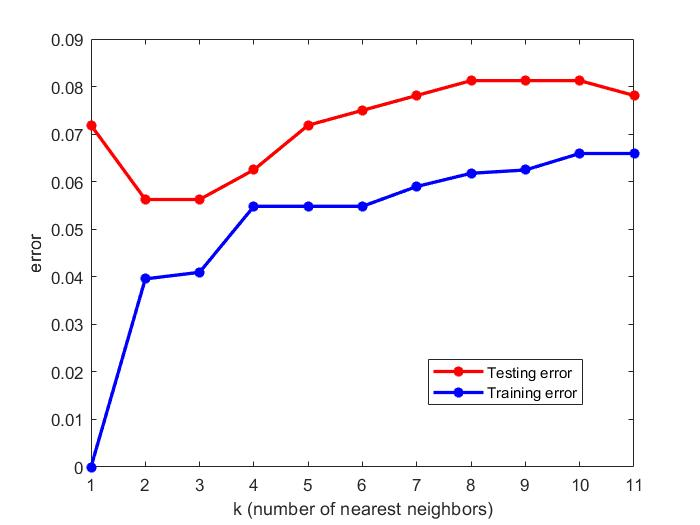
\includegraphics[width=.9\linewidth]{figures/knnerror.jpg}
		\caption{Error Plot}
		\label{fig:knnerror}
	\end{subfigure}%
	\begin{subfigure}{.38\textwidth}
		\centering
		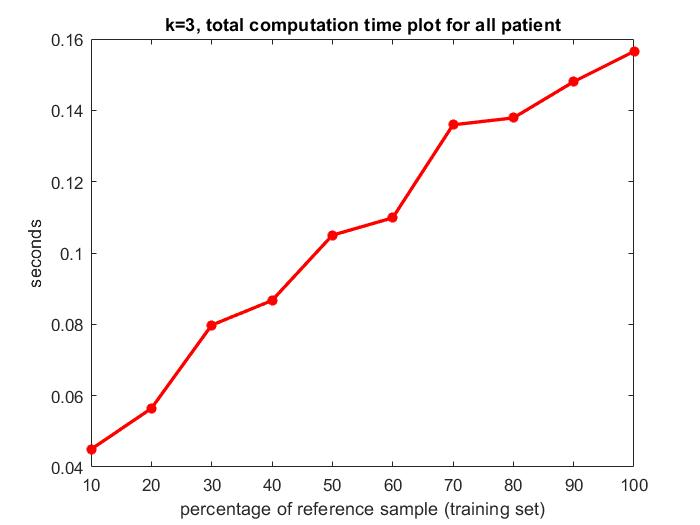
\includegraphics[width=.9\linewidth]{figures/kNNpercentage.jpg}
		\caption{Computation Time}
		\label{fig:knncomp}
	\end{subfigure}
	\caption{\knn{} performance: training/test errors (left) and 
	computation time (right).}
	\label{fig:knn}
\end{figure}

%\begin{figure}[t]
%	\centering
%	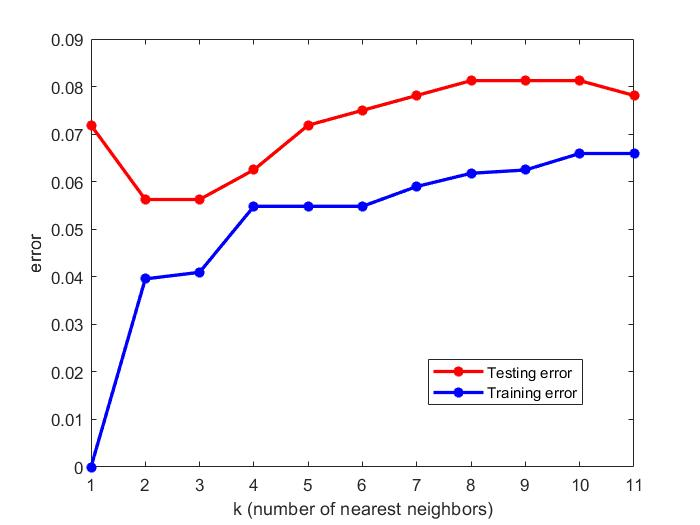
\includegraphics[width=0.6\textwidth]{figures/knnerror.jpg}
%	\caption{Error Plot}
%	\label{fig:knnerror}
%\end{figure}

%\begin{figure}[t]
%	\centering
%	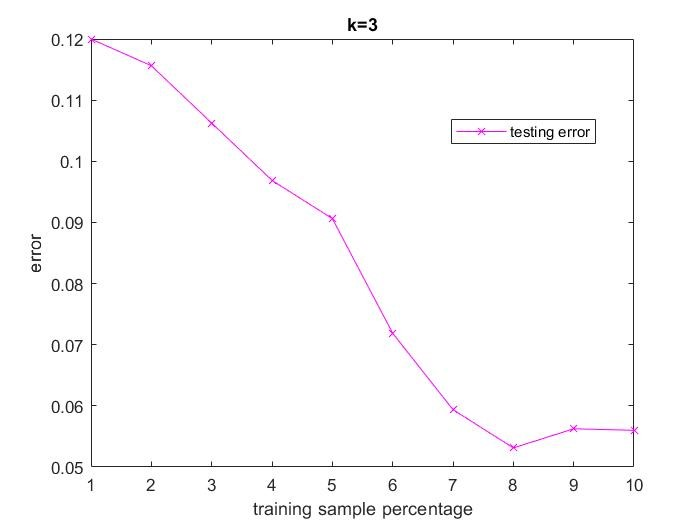
\includegraphics[width=0.6\textwidth]{figures/knntest.jpg}
%	\caption{Test Error}
%	\label{fig:knntest}
%\end{figure}

%\begin{figure}[t]
%	\centering
%	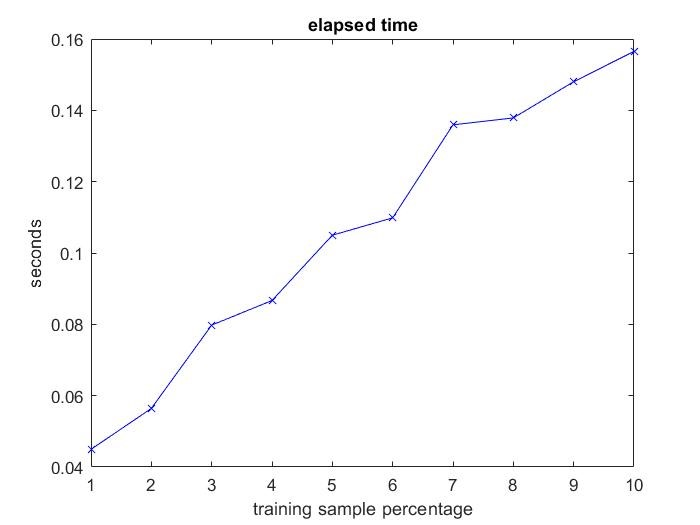
\includegraphics[width=0.6\textwidth]{figures/knncomp.jpg}
%	\caption{Computation Time}
%	\label{fig:knncomp}
%\end{figure}




%Figure~\ref{fig:knntest} shows that the test error decreases as the 
%training set becomes larger.










\section{Experimental results and Discussion}
\label{sec:res}
The performance measures for all algorithms is presented in a 
Table~\ref{tbl:res}

\begin{table}[]
	\begin{center}
	\begin{tabular}{|l|l|c|c|c|c|}
		\hline
		\multicolumn{2}{|l|}{}                                        
		                            & 
		\multicolumn{1}{l|}{\textbf{DNN}} & 
		\multicolumn{1}{l|}{\textbf{Decision tree}} & 
		\multicolumn{1}{l|}{\textbf{SVM}} & 
		\multicolumn{1}{l|}{\textbf{k-NN}} \\ \hline
		\multicolumn{2}{|l|}{\textbf{Accuracy 
		0-1}}                                               & 
		0.9344                            &                           
		                  &                                   
		&                                    \\ \hline
		\multicolumn{2}{|l|}{\textbf{Sensitivity}}                    
		                            & 
		0.9125                            &                           
		                  &                                   
		&                                    \\ \hline
		\multicolumn{2}{|l|}{\textbf{Specificity}}                    
		                            & 
		0.9563                            &                           
		                  &                                   
		&                                    \\ \hline
		\multicolumn{2}{|l|}{\textbf{Precision}}                      
		                            & 
		0.9542                            &                           
		                  &                                   
		&                                    \\ \hline
		\multicolumn{2}{|l|}{\textbf{F1}}                             
		                            & 
		0.933                             &                           
		                  &                                   
		&                                    \\ \hline
		\multirow{4}{*}{\begin{tabular}[c]{@{}l@{}}Confusion\\ 
		matrix\end{tabular}} & \textbf{TP} 
		&                                   &                         
		                    &                                   
		&                                    \\ \cline{2-6} 
		& \textbf{TN} &                                   
		&                                             &               
		                    &                                    \\ 
		\cline{2-6} 
		& \textbf{FP} & 7/160                             
		&                                             &               
		                    &                                    \\ 
		\cline{2-6} 
		& \textbf{FN} & 14/160                            
		&                                             &               
		                    &                                    \\ 
		\hline
		\multicolumn{2}{|l|}{\textbf{Test time (per 
		patient)}}                                    &               
		                    
		&                                             &               
		                    &                                    \\ 
		\hline
		\multicolumn{2}{|l|}{\textbf{Probability 
		estimation}}                                     & 
		+                                 &                           
		                  &                                   
		&                                    \\ \hline
	\end{tabular}
\end{center}
\caption{BLA}
\label{tbl:res}
\end{table}

DISCUSSION ON THE RESULTS GOES HERE
\section*{Acknowledgments}
\label{sec:ack}
The authors would like to thank Kuk Jin Jang for the valuable 
discussion on the existing arrhythmia monitoring algorithms and 
publicly available ECG databases. 

\newpage
\bibliographystyle{plain}
\bibliography{project_bib} 
\end{document}


